\section{Introduzione}
La valutazione euristica nasce intorno agli anni '90, ad opera del lavoro di Jakob Nielsen e Donald Norman\footnote{fonte Wikipedia}; tale metodo si basa sull'assunto che non vi sia interazione con gli utenti, ma � il frutto del lavoro di un team d'esperti che valutano il sito web, o pi� in generale una qualsivoglia applicazione, secondo una serie di principi prefissati. L'obiettivo � individuare e catalogare i problemi di usabilit�, al fine di trovare una soluzione che sia la pi� adatta possibile, innalzando cos� il livello qualitativo dell'applicazione stessa.\\
\'E chiaro che la scelta dei principi � punto cruciale: si possono trovare vari insiemi e tutti possono dare risultare soddisfacenti, ma con sfumature diverse; � altrettato ovvio che si deve cercare di applicare l'insieme di principi adatto al contesto dell'applicazione. Nel nostro caso abbiamo scelto di utilizzare quelli proposti da Nielsen per varie ragioni, che verranno spiegate nelle sezioni sucessive.\\
La valutazione euristica prevede che ogni membro del team di valutatori lavori da solo al fine da evitare reciproca influenza o condizionamento. \'E riscontrato che lavorando da soli si affrontano problematiche diverse alle quali si da un peso diverso a seconda dell'esperienza personale del valutatore, pertanto � fondamentale che non vi siano interferenze di nessun genere durante questa fase.\\
Da questo assunto si pu� dedurre che i valutatori possano trovare problematiche differenti. Tuttavia il numero di errori scoperti non cresce linearmente col numero di valutatori, fino al raggiungimento del 100\% di errori trovati, ma vi si avvicina in maniera asintotica. Osservando la figura \ref{fig:grafico_curva_errori} si pu� notare come l'incremento della percentuale di errori trovati inizialmente diminuisca in fretta all'aumentare del numero di valutatori, rallentando man mano. Bastano infatti solamente cinque esaminatori per individuare il 75\% degli errori complessivi, mentre raddoppiando il numero di valutatori, la percentuale di errori trovati si incrementa solo di una decina di punti circa.\\ 
\begin{figure}[!h]
\centering
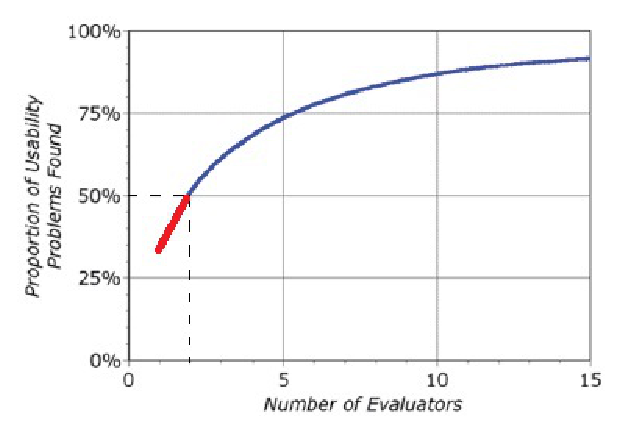
\includegraphics[scale=0.85]{figure/grafico_valutatori_errori.eps}
\caption{Curva teorica di Nielsen che lega il numero di valutatori ed il
numero di problemi individuati.} \label{fig:grafico_curva_errori}
\end{figure}\\
Il grafico sopracitato, � esprimibile mediante l'equazione:
\begin{equation}
problemi = M (1- (1-L)^{N}) \nonumber
\end{equation}
i cui parametri rappresentano:
\begin{itemize}
\item M = numero d problemi totali;
\item L = percentuale di errori trovati da ogni valutatore, che secondo; alcuni esperimenti empirici di Nielsen, si aggira intorno al 31\%
\item N = numero totale di esamitatori coinvolti nella valutazione.
\end{itemize}
Per organizzare i vari lavori da svolgere e avere una certa omogeneit� e coerenza durante il procedimento degli stessi � necessaria una fase di pianificazione del lavoro, tempistiche, modalit� (fase di {\it briefing}). In genere l'analisi euristica si compone di una o pi� sessioni di valutazione che hanno una durata circa di 1-2 ore ciascuna, durante la quale ogni esaminatore valuta l'applicazione, elencando le varie problematiche, il grado di critici�, e quale o quali principi vengono violati. Terminata questa seconda fase, si passa alla fusione delle varie valutazioni, uniformando cos� la lista degli errori (fase di {\it debriefing}); � chiaro che quest'operazione possa essere facilmente ottimizzata affiancando uno stesso {\it osservatore} per ogni esaminatore, in tal modo si mantiene la lista delle violazioni ai principi precedentemente adottati uniforme, poich� � una sola persona a compilarla.\\
Dalle constatazioni fino ad ora emerse, possiamo dedurre che la valutazione euristica � uno strumento assai potente ed efficiente; richiede tempi di elaborazione modesti e fornisce risultati di ottima qualit�.\\
Di contro in genere non fornisce alcun tipo di soluzione, pertanto richiede un successivo lavoro d'integrazione al fine di proporre delle valide soluzioni per i problemi riscontrati. 
